\chapter{Déterminants}

À chaque matrice carrée $\matA$, on peut associer un scalaire, appelé le \definition{déterminant} de la matrice
et dénoté soit par $\det(\matA)$ ou par $|\matA|$.  Nous avons la même notation lorsque nous avons
une matrice sous forme explicite:
\[
\det\begin{pmatrix}
a & b \\
c & d
\end{pmatrix}
=
\begin{vmatrix}
a & b \\
c & d
\end{vmatrix}
\]
Le déterminant d'une matrice $1\times  1$ est simplement le coefficient:
\[
\det(a) = |a| = a
\]
À noter qu'en dépit de la notation des barres verticales, il ne s'agit pas d'une
valeur absolue!   
Dans ce qui suit, nous allons définir le déterminant d'un manière
récursive, à partir de la définition ci-dessus pour une matrice $1\times  1$.
Mais, auparavant, il est utile de définir deux termes.

\section{Mineur et cofacteur}
Soit une matrice carrée $\matA$ de taille $n\times  n$.
Soit $\mat{M}_{ij}$ la matrice carrée $(n-1)\times (n-1)$ obtenue en
supprimant la ligne $i$ et la colonne $j$ de $\matA$.
\begin{exemple}
Soit la matrice \[\displaystyle \matA = \begin{pmatrix}
1 & 2 & 3\\
4 & 5 & 6 \\
7 & 8 & 9
\end{pmatrix}\].
À partir de cette matrice, en éliminant une ligne et une colonne, on peut définir 9 matrices dont
les trois suivantes:
 \[
 \mat{M}_{11} = \begin{pmatrix}
  & \tikzmark{a11}1 & 2 & 3 \tikzmark{b11}&\\
 & \tikzmark{c11}4 & 5 & 6 \\
 & 7 \tikzmark{d11}& 8 & 9
 \end{pmatrix}
 = \begin{pmatrix}
 5 & 6 \\
 8 & 9
 \end{pmatrix}
  \DrawBox[white,pattern=north east lines, pattern color=red]{a11}{b11}
  \DrawBox[white,pattern=north east lines, pattern color=red]{c11}{d11}
\]

 \[
 \mat{M}_{12} = \begin{pmatrix}
  & \tikzmark{a12}1 & 2 & 3 \tikzmark{b12}&\\
 & 4 & \tikzmark{c12} 5 & 6 \\
 & 7 & 8 \tikzmark{d12}& 9
 \end{pmatrix}
 = \begin{pmatrix}
 4 & 6 \\
 7 & 9
 \end{pmatrix}
  \DrawBox[white,pattern=north east lines, pattern color=red]{a12}{b12}
  \DrawBox[white,pattern=north east lines, pattern color=red]{c12}{d12}
\]

 \[
 \mat{M}_{33} = \begin{pmatrix}
  & 1 & 2 &\tikzmark{c33}  3 &\\
 & 4 & 5& 6\tikzmark{d33}  \\
 & \tikzmark{a33}7 & 8 & 9\tikzmark{b33}
 \end{pmatrix}
 = \begin{pmatrix}
 1 & 2 \\
 4 & 5
 \end{pmatrix}
  \DrawBox[white,pattern=north east lines, pattern color=red]{a33}{b33}
  \DrawBox[white,pattern=north east lines, pattern color=red]{c33}{d33}
\]
\end{exemple}

\begin{defini}
Soit une matrice carrée $\matA = (a_{ij})$ de taille $n\times  n$.
On appelle le \Definition{mineur} de l'élément $a_{ij}$ le déterminant de la matrice carrée $\mat{M}_{ij}$  obtenue en
supprimant la ligne $i$ et la colonne $j$ de $\matA$. 
\end{defini}

\begin{exemple}
\label{exemple:det1}
Soit la matrice $\displaystyle \matA = \begin{pmatrix}
1 & 2 & 3\\
4 & 5 & 6 \\
7 & 8 & 9
\end{pmatrix}$.
À partir de cette matrice, en éliminant une ligne et une colonne, on peut définir 9 mineurs
associés au neufs éléments $a_{ij}$ tel qu'illustré par les trois exemples suivants:
 \[
 a_{11} \rightarrow |\mat{M}_{11} | = \begin{vmatrix}
  & \tikzmark{am11}1 & 2 & 3 \tikzmark{bm11}&\\
 & \tikzmark{cm11}4 & 5 & 6 \\
 & 7 \tikzmark{dm11}& 8 & 9
 \end{vmatrix}
 = \begin{vmatrix}
 5 & 6 \\
 8 & 9
 \end{vmatrix}
  \DrawBox[white,pattern=north east lines, pattern color=red]{am11}{bm11}
  \DrawBox[white,pattern=north east lines, pattern color=red]{cm11}{dm11}
\]

 \[
 a_{12} \rightarrow |\mat{M}_{12} | = \begin{vmatrix}
  & \tikzmark{am12}1 & 2 & 3 \tikzmark{bm12}&\\
 & 4 & \tikzmark{cm12} 5 & 6 \\
 & 7 & 8 \tikzmark{dm12}& 9
 \end{vmatrix}
 = \begin{vmatrix}
 4 & 6 \\
 7 & 9
 \end{vmatrix}
  \DrawBox[white,pattern=north east lines, pattern color=red]{am12}{bm12}
  \DrawBox[white,pattern=north east lines, pattern color=red]{cm12}{dm12}
\]

 \[
 a_{33} \rightarrow |\mat{M}_{33} | = \begin{vmatrix}
  & 1 & 2 &\tikzmark{cm33}  3 &\\
 & 4 & 5& 6\tikzmark{dm33}  \\
 & \tikzmark{am33}7 & 8 & 9\tikzmark{bm33}
 \end{vmatrix}
 = \begin{vmatrix}
 1 & 2 \\
 4 & 5
 \end{vmatrix}
  \DrawBox[white,pattern=north east lines, pattern color=red]{am33}{bm33}
  \DrawBox[white,pattern=north east lines, pattern color=red]{cm33}{dm33}
\]
\end{exemple}

\begin{exerciceC}
Obtenez les 6 autres mineurs pour l'\refexemple{exemple:det1}.
\end{exerciceC}

\begin{defini}
Soit une matrice carrée $\matA = (a_{ij})$ de taille $n\times  n$.
On appelle le \Definition{cofacteur} de l'élément $a_{ij}$, dénoté par $\Cof_{ij}(\matA)$, le déterminant de la matrice carrée $\mat{M}_{ij}$  obtenue en
supprimant la ligne $i$ et la colonne $j$ de $\matA$ multiplié par le facteur $(-1)^{i+j}$. 
\[
\Cof_{ij}(\matA) = (-1)^{i+j} |\mat{M}_{ij}|
\]
\end{defini}
\textbf{Remarques:}
\begin{enumerate}
\item Le cofacteur, $\Cof_{ij}(\matA)$, est un scalaire, et que $\mat{M}_{ij}$ est une matrice.
\item Les facteurs de $(-1)^{i+j}$ sont dans une forme d'échiquier dans une matrice, avec les $+$ sur la diagonale principale
\[
\begin{pmatrix}
+ & - & + & - & \ldots \\
- & + & - & + & \ldots \\
+ & - & + & - & \ldots \\
- & + & - & + & \ldots \\
\vdots & \vdots & \vdots & \vdots & \ddots
\end{pmatrix}
\]
\end{enumerate}

\begin{exemple}
\label{exemple:det2}
Soit la matrice $\displaystyle \matA = \begin{pmatrix}
1 & 2 & 3\\
4 & 5 & 6 \\
7 & 8 & 9
\end{pmatrix}$.
À partir de cette matrice, en éliminant une ligne et une colonne, on peut définir 9 cofacteurs
associés au neufs coefficients de la matrice  tel qu'illustré par les trois exemples suivants
\footnote{Comme nous n'avons pas encore défini le déterminant d'une matrice $2\times  2$,
nous ne pouvons pas compléter entièrement les calculs.}
 \[
\Cof_{11}(\matA) = (-1)^{1+1} |\mat{M}_{11} | = \begin{vmatrix}
  & \tikzmark{am11}1 & 2 & 3 \tikzmark{bm11}&\\
 & \tikzmark{cm11}4 & 5 & 6 \\
 & 7 \tikzmark{dm11}& 8 & 9
 \end{vmatrix}
 = \begin{vmatrix}
 5 & 6 \\
 8 & 9
 \end{vmatrix}
  \DrawBox[white,pattern=north east lines, pattern color=red]{am11}{bm11}
  \DrawBox[white,pattern=north east lines, pattern color=red]{cm11}{dm11}
\]

 \[
\Cof_{12}(\matA)  = (-1)^{1+2}  =- |\mat{M}_{12} | = \begin{vmatrix}
  & \tikzmark{am12}1 & 2 & 3 \tikzmark{bm12}&\\
 & 4 & \tikzmark{cm12} 5 & 6 \\
 & 7 & 8 \tikzmark{dm12}& 9
 \end{vmatrix}
 = -\begin{vmatrix}
 4 & 6 \\
 7 & 9
 \end{vmatrix}
  \DrawBox[white,pattern=north east lines, pattern color=red]{am12}{bm12}
  \DrawBox[white,pattern=north east lines, pattern color=red]{cm12}{dm12}
\]

 \[
 \Cof_{33}(\matA)  = (-1)^{3+3} = |\mat{M}_{33} | = \begin{vmatrix}
  & 1 & 2 &\tikzmark{cm33}  3 &\\
 & 4 & 5& 6\tikzmark{dm33}  \\
 & \tikzmark{am33}7 & 8 & 9\tikzmark{bm33}
 \end{vmatrix}
 = \begin{vmatrix}
 1 & 2 \\
 4 & 5
 \end{vmatrix}
  \DrawBox[white,pattern=north east lines, pattern color=red]{am33}{bm33}
  \DrawBox[white,pattern=north east lines, pattern color=red]{cm33}{dm33}
\]
\end{exemple}

\begin{exerciceC}
Obtenez les 6 autres cofacteurs pour l'\refexemple{exemple:det2}.
\end{exerciceC}

\section{Le déterminant}

\begin{defini}
Le \Definition{déterminant} d'une matrice $\matA = (a_{ij})$ carrée de taille $n\times  n$ 
est égal\footnote{\textbf{Remarque:} Dans la majorité des livres, on choisit une autre définition du déterminant d'une matrice, basé
sur des permutations, et on présente la définition ci-dessus comme un théorème qui en découle.  
Dans la pratique, puisqu'on utilise
la définition ci-dessus pour calculer les déterminants, il nous semble plus logique de l'introduire directement
et de passer outre à la définition \textit{standard}.}
 à la somme des produits 
de tous les coefficients d'une ligne (ou d'une colonne) quelconque par leur cofacteurs respectifs:
\[
|\matA| = a_{p1} \Cof_{p1}(\matA)+ a_{p2} \Cof_{p2}(\matA)+ \ldots + a_{pn} \Cof_{pn}(\matA)= \sum_{i=1}^n a_{pi} \Cof_{pi}(\matA)
\]
ou
\[
|\matA| = a_{1\ell} \Cof_{1\ell}(\matA) + a_{2\ell} \Cof_{2\ell}(\matA)+ \ldots + a_{n\ell} \Cof_{n\ell}(\matA) = \sum_{j=1}^n a_{j\ell} \Cof_{j\ell}(\matA)
\]
\end{defini}

\subsection{Les matrices $2\times 2$}
Dans plusieurs livres, on donne la valeur du déterminant d'une matrice $2\times 2$ essentiellement comme 
une définition et on utilise cette valeur pour calculer les déterminants des matrices $n\times  n$.  
Nous avons choisi plutôt d'utiliser directement la définition du déterminant pour obtenir, à partir de la
valeur du déterminant pour une matrice $1\times 1$ celle d'une matrice $2\times 2$.  De plus, comme la définition
du déterminant indique qu'on peut choisir n'importe quelle ligne ou n'importe quelle colonne, nous allons considérer
séparément les 4 cas pour illustrer que le résultat est le même peu importe le choix qu'on fait.  Nous commençons par
calculer les quatres cofacteurs de la matrice générale en terme du déterminant d'une matrice\footnote{Nous rappelons qu'il ne
faut pas confondre les deux barres verticales du déterminant avec une valeur absolue.} $1\times 1$.
\[
\matA = \begin{pmatrix}
a & b \\
c & d
\end{pmatrix}
\]
\[
\Cof_{11}(\matA) = (-1)^{1+1} \begin{vmatrix}
&\tikzmark{a}a& b\tikzmark{b} &\\
&\tikzmark{c}c\tikzmark{d}& d
\end{vmatrix}
= \hphantom{-}|d| = \hphantom{-}d
  \DrawBox[white,pattern=north east lines, pattern color=red]{a}{b}
  \DrawBox[white,pattern=north east lines, pattern color=red]{c}{d}
\]
\[
\Cof_{12}(\matA) = (-1)^{1+2} \begin{vmatrix}
&\tikzmark{a}a & b\tikzmark{b}& \\
&c  &\tikzmark{c} d\tikzmark{d}
\end{vmatrix}
= -|c| = -c
  \DrawBox[white,pattern=north east lines, pattern color=red]{a}{b}
  \DrawBox[white,pattern=north east lines, pattern color=red]{c}{d}
\]
\[
\Cof_{21}(\matA) = (-1)^{2+1} \begin{vmatrix}
&\tikzmark{a}a & b &\\
 &c\tikzmark{b} &\tikzmark{c} d\tikzmark{d}
\end{vmatrix}
= -|b| = -b
  \DrawBox[white,pattern=north east lines, pattern color=red]{a}{b}
  \DrawBox[white,pattern=north east lines, pattern color=red]{c}{d}
\]
\[
\Cof_{22}(\matA) = (-1)^{2+2} \begin{vmatrix}
&a &\tikzmark{a}b\tikzmark{b} &\\
&\tikzmark{c}c & d\tikzmark{d} 
\end{vmatrix}
= \hphantom{-}|a| = \hphantom{-}a
  \DrawBox[white,pattern=north east lines, pattern color=red]{a}{b}
  \DrawBox[white,pattern=north east lines, pattern color=red]{c}{d}
\]
Calculons maintenant le déterminant.  En premier, nous le faisons en
utilisant la première ligne:
\[
|\matA| = a_{11}\Cof_{11}(\matA) + a_{12}\Cof_{12}(\matA) = ad + b(-c) = ad-bc
\]
En utilisant la deuxième ligne:
\[
|\matA| = a_{21}\Cof_{21}(\matA)+ a_{22}\Cof_{22}(\matA)= c(-b) + da = ad-bc
\]
En utilisant la première colonne:
\[
|\matA| = a_{11}\Cof_{11}(\matA) + a_{21}\Cof_{21}(\matA)= ad + c(-b) = ad-bc
\]
En utilisant la deuxième colonne:
\[
|\matA| = a_{12}\Cof_{12}(\matA) + a_{22}\Cof_{22}(\matA)= b(-c) + ad = ad-bc
\]
Nous voyons que le résultat est identique dans tous les cas.  À partir de maintenant, nous allons utiliser ce résultat
directement et toujours calculer les déterminants de manière récursive jusqu'à ce qu'on arrive à des combinaisons
de déterminants de matrices $2\times 2$.

\begin{exerciceC}
Calculez le déterminant de la matrice
\[
\begin{pmatrix}
c & c \\
6 & 2c
\end{pmatrix}
\]
où $c$ est un scalaire.  Pour quelle(s) valeur(s) de $c$ est-ce que le déterminant sera égal à zéro?
\end{exerciceC}


\subsection{Deux exemples de matrice de taille supérieure}

Nous allons considérer deux exemples pour illustrer le calcul de déterminants avant de
considérer certaines propriétés des déterminants dans la section suivante.
\begin{exemple}
Calculons le déterminant de la matrice $
\displaystyle \matA = \begin{pmatrix}
1 & 2 & 3 \\
4 & 5 & 6 \\
7 & 8 & 9
\end{pmatrix}
$
En choisissant de faire l'expansion à partir de la première ligne, nous avons:
\[
\begin{matrix}[rclllll]
|A| =
\begin{vmatrix}
1 & 2 & 3 \\
4 & 5 & 6 \\
7 & 8 & 9
\end{vmatrix}
&=& \begin{vmatrix}
5 & 6 \\
8 & 9
\end{vmatrix}
&-&2 \begin{vmatrix}
4 & 6 \\
7 & 9
\end{vmatrix}
&+&3 \begin{vmatrix}
4 & 5 \\
7 & 8
\end{vmatrix}
\\
&=& (5\cdot 9 - 6\cdot 8) &-&2(4\cdot9 - 6\cdot7) &+& 3(4\cdot8 - 5\cdot7) \\
&=& -3 & +&12 & -&9 \\
&=& 0
\end{matrix}
\]
\end{exemple}

\begin{exemple}
\label{ex:mat4}
Calculez le déterminant de la matrice $
\displaystyle\matA = \begin{pmatrix}
4 & 5 & 3 & 3 \\
0 & 0 & 2 & 0 \\
2 & 6 & 7 & 0 \\
8 & 4 & 9 & 0
\end{pmatrix}
$
\solution
Puisqu'il s'agit d'une matrice $4\times 4$, nous pouvons écrire le déterminant
comme une somme de 4 termes, chacun contenant un déterminant d'une
matrice $3\times 3$.  Pour réduire la quantité de calcul qu'on doit faire, on
note que, si on choisit de faire l'expansion suivant la deuxième ligne, trois
des quatres termes seront zéros parce que chaque terme sera multiplié par
le coefficient 0.  Donc, le déterminant de $\matA$ est
\[
\begin{vmatrix}
4 & 5 & 3 & 3 \\
0 & 0 & 2 & 0 \\
2 & 6 & 7 & 0 \\
8 & 4 & 9 & 0
\end{vmatrix}
= -2 \begin{vmatrix}
4 & 5 & 3 \\
2 & 6 & 0 \\
8 & 4 & 0
\end{vmatrix}
\] 
On note ici que la troisième colonne ne contient qu'un coefficient différent de zéro.
Nous choisissons donc cette colonne pour faire l'expansion suivante:
\[
|\matA|
= (-2)(3) \begin{vmatrix}
2 & 6  \\
8 & 4 
\end{vmatrix} = (-2)(3)(2\cdot4-6\cdot8) = 240
\]
\end{exemple}
\begin{exerciceC}
Calculez le déterminant de la matrice de l'exemple précédent en faisant d'abord l'expansion
suivant la première ligne.
\end{exerciceC}
\section{Propriétés des déterminants}

\subsection{Matrices diagonales et triangulaires}
\begin{theo}
\parttheorem{a} Le déterminant de la matrice identité $I_n$ est égal à 1.
\parttheorem{b} Le déterminant d'une matrice diagonale $\matD$ est le produit des
éléments de la diagonale: 
\[
\det \matD = \prod_{i=1}^n d_{ii}
\]
\parttheorem{c} Le déterminant d'une matrice triangulaire est le produit des éléments
de la diagonale.
\proof
Nous allons prouver ces propriétés par induction. On démontre tout d'abord que c'est
vrai dans le cas $n=1$, ou $n=2$, puis, on suppose que c'est vrai dans le cas $n-1$ pour démontrer
que ceci implique que c'est vrai pour $n$.
\parttheorem{a} Le déterminant de $I_1 = (1) = 1$.  Il Considérons le déterminant de
la matrice $I_n$:
\[
|I_n| = \begin{vmatrix}[lc]
1 & \begin{matrix} 0 & \ldots \end{matrix}\\
\begin{matrix}
0 \\
\vdots
\end{matrix} & I_{n-1} 
\end{vmatrix}
\]
En faisant le développement par la première ligne (ou par la première colonne!), on trouve:
\[
|I_n| = |I_{n-1}|
\]
Mais puisque, par hypothèse, $|I_{n-1}|=1$, cela implique que $|I_n|=1$. \cqfd
\parttheorem{b} Le déterminant de $D_1 = (d_{11}) = d_{11}$.  Le déterminant
de $D_2$ est:
\[
\begin{vmatrix}
d_{11} & 0 \\
0 & d_{22}
\end{vmatrix} = d_{11}d_{22} - 0 = \prod_{i=1}^2 d_{ii}
\]
Considérons le déterminant de la matrice $D_n$:
\[
|D_n| = \begin{vmatrix}[lc]
d_{11} & \begin{matrix} 0 & \ldots \end{matrix}\\
\begin{matrix}
0 \\
\vdots
\end{matrix} & D_{n-1} 
\end{vmatrix}
\]
En faisant le développement par la première ligne (ou par la première colonne!), on trouve:
\[
|D_n| = d_{11}|D_{n-1}|
\]
Mais puisque, par hypothèse, $\displaystyle |D_{n-1}|=\prod_{i=1}^{n-1}$, cela implique que 
$\displaystyle |D_n|=\prod_{i=1}^2 d_{ii}$. \cqfd
\parttheorem{c} La preuve, qui est semblable à la précédente, est laissée à faire en exercice.
\end{theo}

\begin{exerciceC}
Prouvez que le déterminant d'une matrice triangulaire est le produit des éléments
de la diagonale.
\end{exerciceC}

\subsection{Matrice ayant une colonne ou une ligne nulle}

\begin{theo}
Si une matrice carrée $\matA$ a une ligne ou une colonne remplie de zéros, alors $|\matA|=0$.
\proof:
Il suffit de faire l'expansion du déterminant selon la ligne (ou la colonne) qui est remplie de zéros.
\end{theo}

\subsection{Transposée}
\begin{theo}
Le déterminant d'une matrice est égal au déterminant de sa transposée: $|\matA| = |\transp{\matA}|$.
\proof
Écrivons $\matB = \transp{\matA}$. Si l'on compare le déterminant de $\matA$ selon la ligne $j$:
\[
|\matA| = \sum_{\ell=1}^n a_{j\ell} \Cof_{j\ell}(\matA)
\]
avec le déterminant de sa transposée selon la colonne $j$:
\[
|\transp{\matA}| =|\matB| = \sum_{\ell=1}^n b_{\ell j} \Cof_{\ell j}(\matB)
\]
on constate qu'ils sont égaux puisque $b_{\ell j} = a_{j \ell}$ et similairement
$\Cof_{\ell j}(\matB) = \Cof_{j\ell}(\matA)$ par la définition de la transposée.
\end{theo}

\subsection{Matrice élémentaires}

Avant de continuer à prouver diverses propriétés, nous allons calculer le déterminant de trois matrices 
élémentaires $2\times 2$.  Tout d'abord, nous calculons le déterminant de la matrice qui, 
lorsqu'on la multiplie à une autre matrice de la même taille, correspond à multiplier la première rangée par une 
constante:
\[
|\matE_1(k)| = \begin{vmatrix}
k & 0\\
0 & 1
\end{vmatrix} = k
\]
Ensuite, nous calculons le déterminant de la matrice qui correspond à l'échange de deux lignes:
\[
|\matE_{1 \leftrightarrow 2}| = \begin{vmatrix}
0 & 1\\
1 & 0
\end{vmatrix} = 0-1 = -1
\]
Finalement, nous calculons le déterminant de la matrice qui correspond à remplacer la première ligne par l'addition d'elle-même à  $k$ fois la deuxième ligne:
\[
|\matE_{12}(k)| = \begin{vmatrix}
1 & k \\
0 & 1
\end{vmatrix} = 1 - k\cdot 0 = 1
\]
On note qu'il y a une quatrième possibilité, soit $\matE_{21}(k)$ mais 
\[
\left|\matE_{21}(k)\right| = \left|\transp{\matE}_{12}(k)\right| =\left|\matE_{12}(k)\right| = 1
\]
où nous avons utilisé le fait que le déterminant de la transposée d'une matrice est égal au déterminant de la matrice elle-même.

Maintenant, nous sommes prêt à calculer le déterminant du produit de telles matrices.  Soit une matrice $\matA$ de taille $2\times 2$ avec des coefficients arbitraires:
\[
\matA = \begin{pmatrix}
a & b \\
c & d
\end{pmatrix}
\]
Son déterminant est $ad-bc$.  Maintenant, évaluons le produit d'une des trois matrices élémentaires précédentes par cette matrice. Nous allons vérifier que, dans chacun des trois cas, $|\matE \matA| = |\matE| |\matA|$.
\[
\left|\matE_1(k) \matA \right| =  \left|\begin{pmatrix}
k & 0 \\
0 & 1
\end{pmatrix}
\begin{pmatrix}
a & b \\
c & d
\end{pmatrix} \right|
= \begin{vmatrix}
ka & kb \\
c & d
\end{vmatrix} = kad - kbc = k(ad-bc) = |\matE_1(k)| |\matA|
\]
%
\[
\left|\matE_{1\leftrightarrow 2} \matA \right| =  \left|\begin{pmatrix}
0 & 1 \\
1 & 0
\end{pmatrix}
\begin{pmatrix}
a & b \\
c & d
\end{pmatrix} \right|
= \begin{vmatrix}
c & d \\
a & b
\end{vmatrix} = bc - ad = -(ad-bc) = |\matE_{1\leftrightarrow 2} | |\matA|
\]
%
\begin{eqnarray*}
\left|\matE_{12}(k) \matA \right| =  \left|\begin{pmatrix}
1 & k \\
0 & 1
\end{pmatrix}
\begin{pmatrix}
a & b \\
c & d
\end{pmatrix} \right|
= \begin{vmatrix}
a+kc & b+kd \\
c & d
\end{vmatrix} &=&(a+kc)d - (b+kd)c \\
 &=& ad-bc = |\matE_{12}(k) | |\matA|
\end{eqnarray*}
Pour les matrices élémentaires $n\times  n$, nous avons:
\begin{enumerate}
\item Les matrices $\matE_{i}(k)$ sont des matrices diagonales; 
leur déterminant est le produit des coefficients diagonaux qui sont tous égaux à 1 sauf pour celui de la ligne $i$ qui est égal à $k$. Donc, leur déterminant est $k$.
\item Les matrices $\matE_{ij}(k)$ sont des matrices triangulaires; 
leur déterminant est le produit des coefficients diagonaux qui sont tous égaux à 1. Donc, leur déterminant est 1.
\item À l'exception des lignes $i$ et $j$, les matrices $\matE_{i\leftrightarrow j}$ n'ont que des coefficients égaux à 1 sur la
diagonale.  En faisant l'expansion du déterminant en premier selon ces autres lignes, on trouve le déterminant d'une matrice plus
petite mais du même type, jusqu'à ce qu'on en arrive à une matrice $2\times  2$ du même type, et dont le déterminant est égal à
-1.  Donc, le déterminant des matrices $n\times  n$ de ce type est également -1.
\end{enumerate}
\begin{theo}
Soit $\matA$ une matrice $n\times  n$ quelconque et $\matE$ une matrice élémentaire $n\times  n$. Alors
\[
\det \matE\matA = (\det \matE) (\det \matA)
\]
\proof
Pour démontrer ce résultat, nous allons procéder par induction.  Nous avons déjà vu que ceci était vrai dans le cas $2\times 2$.
Supposons que nous avons vérifié le résultat dans le cas $(n-1)\times (n-1)$ et considérons le cas $n\times  n$.  Le résultat de
multiplier $\matE$ et $\matA$ ensemble est de changer soit une ou deux des lignes de $\matA$.  Considérons une ligne
de $A$, dénotée par $i$ qui n'a pas changée et écrivons $\matE\matA = \matB$.  Nous pouvons faire le calcul du déterminant de $\matA$ selon cette ligne:
\[
\det(\matE\matA) = \det(\matB) =  \sum_{j=1}^n b_{ij} \det \matB_{ij}
\]
Puisque nous considérons une rangée inchangée, dans chaque terme nous avons $b_{ij}=a_{ij}$, ce qui donne
\[
\det(\matE\matA) \sum_{j=1}^n a_{ij} \det \matB_{ij}
\]

Également, dans chaque terme, le mineur $\matB_{ij}$, de taille $(n-1)\times (n-1)$ 
a été obtenu du mineur correspondant $\matA_{ij}$ par une 
opération élémentaire sur les lignes via une multiplication par une matrice élémentaire que 
nous dénotons par $\matE_{(j)}$ et qui est dans chaque cas du même type que
celle opérant sur la matrice $\matA$ originale.  Par hypothèse, nous savons que pour cette matrice de taille 
$(n-1)\times (n-1)$ 
\[
\det \matB_{ij} = \det(\matE_{(j)} )\det(\matA_{ij})
\]
et donc
\[
\det(\matE\matA) = \sum_{j=1}^n a_{ij} (\det\matE_{(j)} )(\det \matA_{ij})
\]
Comme toutes les matrices $\matE_{(j)} $ dans cette somme sont du même type, le déterminant est une constante
qui a la même valeur que le déterminant de la matrice $\matE$ originale; cette constante
peut être sortie de la somme et nous avons:
\[
\det(\matE\matA) = (\det\matE)\sum_{j=1}^n a_{ij} (\det \matA_{ij}) = (\det\matE)(\det\matA)
\]
\cqfd
\end{theo}

\textbf{Corollaire:} Si on a une matrice qui a deux lignes identiques (ou deux colonnes identiques), son déterminant sera nul.  En effet, on sait que si on interchange les deux
lignes identiques, la matrice ne changera pas mais son déterminant changera de signe.
Le seul scalaire qui est égal à son inverse additif est zéro.

\textbf{Corollaire:} Si on a une matrice dont une ligne est un multiple d'une autre
 (ou dont deux colonnes sont des multiples), son déterminant sera nul.  En effet,il suffit
 de multiplier une ligne par le multiple pour avoir deux lignes identiques; le déterminant
 sera égal à zéro (divisé par le multiple par lequel on aurait multiplié la ligne ou 
 la colonne).


\begin{exerciceC}
Soit la matrice $\matA = \displaystyle \begin{pmatrix}
1 & 2 \\ 3 & 4
\end{pmatrix}$
\partexercice{a} Calculez $\det{\matA}$
\partexercice{b} Si $\matE = \displaystyle \begin{pmatrix}
1 & 2 \\ 0 & 1
\end{pmatrix}$
calculez $\det (\matE\matA)$ et comparez le résultat avec $(\det \matE)( \det\matA)$.
\partexercice{c} Si $\matE = \displaystyle \begin{pmatrix}
0 & 1 \\ 1 & 0
\end{pmatrix}$
calculez $\det (\matE\matA)$ et comparez le résultat avec $(\det \matE)( \det\matA)$.
\partexercice{d} Si $\matE = \displaystyle \begin{pmatrix}
4 & 0 \\ 0 & 1
\end{pmatrix}$
calculez $\det (\matE\matA)$ et comparez le résultat avec $(\det \matE)( \det\matA)$.
\partexercice{e} Calculez $\det (4\matA)$.
\end{exerciceC}

\subsection{Déterminant, produit de matrices et inverse}

\begin{theo}
\label{det0:inv}
Soit $\matA$ et $\matB$ deux matrices $n\times  n$.
\parttheorem{a} Si $\matA$ est inversible, son déterminant est différent de zéro.
\parttheorem{b} Si $\matA$ n'est pas inversible, son déterminant est zéro.
\proof
\parttheorem{a} Si $\matA$ est inversible, on peut obtenir $\matA$ en effectuant des opérations
élémentaires successives à partir de la matrice identité, ou encore
\[
\matA = \matE_1 \matE_2 \ldots \matE_m I_n
\]
En utilisant successivement la propriété $\det(\matE\matB) = (\det\mat E) (\det\matB)$, on peut obtenir:
\[
\det \matA = \det( \matE_1) \det( \matE_2) \ldots \det(\matE_m) \det( I_n)
\]
Comme chacun des déterminants individuels du côté droit de l'équation est différent de zéro, le déterminant
de $\matA$ est différent de zéro.
\parttheorem{b} Si $\matA$ n'est pas inversible, en appliquant successivement des opérations élémentaires, on peut
obtenir une matrice échelonnée $\mat{M}$ dont au moins une rangée est égale à zéro.  Par conséquent, le 
déterminant de cette matrice est zéro.  Nous avons donc
 \[
 \det (\matE_1 \matE_2 \ldots \matE_m \matA) = 
 \det( \matE_1) \det( \matE_2) \ldots \det(\matE_m) \det(\matA) = \det(\mat{M}) = 0
 \]
 Comme le déterminant des matrices élémentaires est différent de zéro, on doit avoir $\det\matA = 0$.
 \cqfd
\end{theo}


\begin{theo}
\parttheorem{a} Soit $\matA$ et $\matB$ deux matrices $n\times  n$.  Le déterminant de leur
produit est égal au produit de leur déterminant:
\[
\det(\matA\matB) = (\det\matA) (\det\matB)
\]
\parttheorem{b} Si $\matA$ est inversible, son déterminant est l'inverse multiplicatif du déterminant de la matrice inverse:
\[
\det(\matA) = \frac{1}{\det\matA^{-1}}
\]
\proof
\parttheorem{a} Nous devons considérez deux cas. 
Premièrement, si $\matA$ n'est pas inversible, alors leur produit $\matA\matB$ n'est également pas inversible
et nous avons trivialement
\[
0 = \det(\matA\matB) =  0 (\det\matB) = (\det\matA) (\det\matB)
\]
Deuxièmement, si $\matA$ est inversible, alors on peut écrire $\matA$ comme un produit de matrice élémentaires multipliées par
la matrice identité:
\[
\matA = \matE_1 \matE_2 \ldots \matE_m \matI_n
\]
et donc
\[
\matA\matB = \matE_1 \matE_2 \ldots \matE_m \matI_n \matB = \matE_1 \matE_2 \ldots \matE_m\matB
\]
En prenant le déterminant de chaque côté, on obtient
\begin{eqnarray*}
\det(\matA\matB) &=& \det(\matE_1\matE_2\ldots \matE_m\matB) \\
&=& (\det\matE_1) (\det\matE_2)\ldots (\det\matE_m) (\det\matB) \\
&=& (\det\matA)(\det\matB)
\end{eqnarray*}
Dans les deux cas, nous avons donc $\det(\matA\matB) (\det\matA) (\det\matB)$.
\cqfd
\parttheorem{b} Il suffit de considérer 
\[
1 = \det\matI = \det(\matA\matA^{-1}) = (\det\matA)(\det\matA^{-1})
\]
d'où
\[
\det(\matA) = \frac{1}{\det\matA^{-1}}
\]
\end{theo}

\begin{exerciceC}
Soit la matrice \[
\matA = \begin{pmatrix}
1 & 1 & 1 \\
1 & 2 & 0 \\
1 & 1 & 2
\end{pmatrix}
\]
Calculez le déterminant de $\matA^7$.
\end{exerciceC}


\subsection{Opérations élémentaires sur les lignes}
Puisque la multiplication par une matrice élémentaire est équivalente à faire des opérations sur les lignes, et vice-versa, on peut se servir de ceci pour calculer les déterminants.  De plus, et ceci est important, comme le déterminant de la transposée d'une matrice est le même que celui de la matrice (non-transposée), on peut,
lors du calcul des déterminants:
\begin{enumerate}
\item transposer une matrice
\item faire une opération élémentaire sur ses lignes
\item transposer la matrice résultante
\end{enumerate}
et ce résultat est équivalent à faire une opération élémentaire sur les \textbf{colonnes} directement, sans
avoir à faire d'abord une transposition puis de terminer par une transposition.

Pour démontrer ceci, reprenons la matrice de
l'\refexemple{ex:mat4}
et calculons le déterminant de la matrice $
\displaystyle\matA = \begin{pmatrix}
4 & 5 & 3 & 3 \\
0 & 0 & 2 & 0 \\
2 & 6 & 7 & 0 \\
8 & 4 & 9 & 0
\end{pmatrix}
$
Nous allons faire ceci en utilisant au maximum les opérations élémentaires sur les lignes (et sur les colonnes).
Nous n'allons pas faire les calculs de la façon la plus efficace: nous allons plutôt faire des transformations
visant à soit faire une expansion (à partir d'une ligne ou d'une colonne) qui n'aura qu'un seul terme avec
le coefficient 1 dans la première ligne et la première colonne, ou soit à extraire au maximum des facteurs
communs pour que l'on ait de petits chiffres à manipuler.  Le but est d'illustrer les diverses opérations possibles.
\[
\begin{vmatrix}
4 & 5 & 3 & 3 \\
0 & 0 & 2 & 0 \\
2 & 6 & 7 & 0 \\
8 & 4 & 9 & 0
\end{vmatrix}
=
\begin{vmatrix}
0 & 1 & 0 & 0 \\
1 & 0 & 0 & 0 \\
0 & 0 & 1 & 0 \\
0 & 0 & 0 & 1
\end{vmatrix}
\begin{vmatrix}
0 & 0 & 2 & 0 \\
4 & 5 & 3 & 3 \\
2 & 6 & 7 & 0 \\
8 & 4 & 9 & 0
\end{vmatrix}
= - 
\begin{vmatrix}
0 & 0 & 2 & 0 \\
4 & 5 & 3 & 3 \\
2 & 6 & 7 & 0 \\
8 & 4 & 9 & 0
\end{vmatrix}
\]
où le signe $-$ vient du déterminant de la matrice élémentaire faisant l'interchange de deux lignes (1 et 2).  
À partir de maintenant, nous n'allons pas écrire la matrice élémentaire requise\footnote{Ou,
dans le cas d'opérations sur les colonnes, les trois opérations requises: 
transposition, opération élémentaire sur les lignes, transposition}
et indiquer seulement le résultat de chaque opération.
\[
\begin{vmatrix}
0 & 0 & 2 & 0 \\
4 & 5 & 3 & 3 \\
2 & 6 & 7 & 0 \\
8 & 4 & 9 & 0
\end{vmatrix}
= - 
\begin{vmatrix}
2& 0 & 0 & 0 \\
3& 5 & 4 & 3 \\
7& 6 & 2 & 0 \\
9& 4 & 8 & 0
\end{vmatrix}
\]
où le signe $-$ vient de l'interchange de deux colonnes (1 et 3).
\[
\begin{vmatrix}
2& 0 & 0 & 0 \\
3& 5 & 4 & 3 \\
7& 6 & 2 & 0 \\
9& 4 & 8 & 0
\end{vmatrix}
= 2 
\begin{vmatrix}
1& 0 & 0 & 0 \\
3& 5 & 4 & 3 \\
7& 6 & 2 & 0 \\
9& 4 & 8 & 0
\end{vmatrix}
\]
où le facteur de 2 vient de la division de la première ligne par 2 (l'opération élémentaire consisterait
à multiplier la première ligne du côté droit par le facteur de 2 pour obtenir le côté gauche de l'équation).  
\textbf{Important:} veuillez noter que lorsqu'on multiplie un déterminant par un scalaire, 
ce n'est pas comme la multiplication d'une matrice par un scalaire: ce n'est pas équivalent
à multiplier tous les coefficients de la matrice par le scalaire; c'est équivalent à multiplier
les coefficients sur une seule ligne (ou une seule colonne) par ce scalaire.

En faisant l'expansion le long de la première ligne, on n'a qu'un terme:
\[
\begin{vmatrix}
1& 0 & 0 & 0 \\
3& 5 & 4 & 3 \\
7& 6 & 2 & 0 \\
9& 4 & 8 & 0
\end{vmatrix}
=  
\begin{vmatrix}
5 & 4 & 3 \\
6 & 2 & 0 \\
4 & 8 & 0
\end{vmatrix}
\]
On peut interchanger la première et la troisième colonne:
\[
\begin{vmatrix}
5 & 4 & 3 \\
6 & 2 & 0 \\
4 & 8 & 0
\end{vmatrix} = -
\begin{vmatrix}
3& 4 & 5 \\
0& 2 & 6 \\
0& 8 & 4
\end{vmatrix}
\]
Si on divise la première \textbf{colonne} par 3, on obtient
\[
\begin{vmatrix}
3& 4 & 5 \\
0& 2 & 6 \\
0& 8 & 4
\end{vmatrix} = 3
\begin{vmatrix}
1& 4 & 5 \\
0& 2 & 6 \\
0& 8 & 4
\end{vmatrix}
\]
En faisant l'expansion par la première colonne, on a
\[
\begin{vmatrix}
1& 4 & 5 \\
0& 2 & 6 \\
0& 8 & 4
\end{vmatrix} = 
\begin{vmatrix}
 2 & 6 \\
 8 & 4
\end{vmatrix}
\]
Finalement, faisons deux opérations, soit de diviser la première ligne par 2 et la deuxième par 4:
\[
\begin{vmatrix}
 2 & 6 \\
 8 & 4
\end{vmatrix} = (2)(4)
\begin{vmatrix}
 1 & 3 \\
 2 & 1
\end{vmatrix}
\]
En résumé, nous avons
\[
\begin{vmatrix}
4 & 5 & 3 & 3 \\
0 & 0 & 2 & 0 \\
2 & 6 & 7 & 0 \\
8 & 4 & 9 & 0
\end{vmatrix}
= (-1)(-1)(2)(-1)(3)(2)(4)
\begin{vmatrix}
 1 & 3 \\
 2 & 1
\end{vmatrix} = -48 [1\cdot 1 - 3\cdot 2] = (-48)(-5) = 240
\]
ce qui est le même résultat que nous avions eu auparavant.  Pour cet exemple-ci, les différentes étapes que nous
avons suivi ont fait en sorte que le calcul a été beaucoup plus long que la façon que nous avions utilisée
précédemment.  Cependant, dans certains cas, les opérations élémentaires sur les lignes permettent de simplifier
beaucoup les calculs ... et sont très utiles si on a de bonnes raisons de croire que le déterminant d'une matrice
est égal à zéro!


\begin{exerciceC}
Soit $|\matA| = \displaystyle \begin{vmatrix}
a & b & c \\
d & e & f \\
g & h & i
\end{vmatrix} = 5$.  Obtenez les déterminants des matrices suivantes. Justifiez vos réponses, soit
comme nous l'avons fait pour la partie \textbf{\color{ExerciceCouleur}(a)} 
dont la réponse est donnée, ou en écrivant une simple phrase indiquant les types d'opérations qui
ont été effectuées.  Veuillez noter que certains déterminants ont été obtenus en faisant plus
qu'une opération.
\partexercice{a} $\displaystyle \begin{vmatrix}
a & b & c \\
2d & 2e & 2f \\
g & h & i
\end{vmatrix}$
\reponse
On peut voir que le déterminant a été obtenu à partir de $|\matA|$ en multipliant la deuxième ligne par 2, ou encore:
\[
\begin{vmatrix}
a & b & c \\
2d & 2e & 2f \\
g & h & i
\end{vmatrix} = 
\begin{vmatrix}
1 & 0 & 0 \\
0 & 2 & 0 \\
0 & 0 & 1
\end{vmatrix}\begin{vmatrix}
a & b & c \\
d & e & f \\
g & h & i
\end{vmatrix} = 2\cdot 5 = 10.
\]
\partexercice{b} $\displaystyle \begin{vmatrix}
a+2d & b+2e & c+2f \\
d & e & f \\
g & h & i
\end{vmatrix}$
\partexercice{c} $\displaystyle \begin{vmatrix}
d & e & f \\
a & b & c \\
g & h & i
\end{vmatrix}$
\partexercice{d} $\displaystyle \begin{vmatrix}
a & d & g \\
b & e & h \\
c & f & i
\end{vmatrix}$
\partexercice{e} $\displaystyle \begin{vmatrix}
a & b & c \\
2d+a & 2e+b & 2f+c \\
g & h & i
\end{vmatrix}$
\partexercice{f} $\displaystyle \begin{vmatrix}
a & 2d & g \\
b & 2e & h \\
c & 2f & i
\end{vmatrix}$
\partexercice{g} $\displaystyle \begin{vmatrix}
a & g& 3d \\
b & h& 3e  \\
c & i& 3f 
\end{vmatrix}$
\end{exerciceC}



\section{Règle de Cramer}
Selon la description de Wikipédia:
\begin{quotation}
\itshape
La \definition{règle de Cramer} (ou méthode de Cramer) est un théorème en algèbre linéaire qui donne la solution d'un système de Cramer, c'est-à-dire un système d'équations linéaires avec autant d'équations que d'inconnues et dont le déterminant de la matrice de coefficients est non nul, en termes de quotients de déterminants.

En calcul, la méthode est moins efficace que la méthode de résolution de Gauss pour des grands systèmes (à partir de 4 équations) dont les coefficients dans le premier membre sont explicitement donnés. Cependant, elle est d'importance théorique pour la raison qu'elle donne une expression explicite pour la solution du système, et elle s'applique dans des systèmes où par exemple les coefficients du premier membre dépendent de paramètres, ce qui peut rendre la méthode de Gauss inapplicable.
\end{quotation}
\begin{defini}
Soit une matrice $\matA$ de taille $n\times  n$. Nous pouvons représenter cette matrice comme une collection
de vecteurs colonnes:
\[
\matA = [\mat{a}_1 \ldots \mat{a}_n]
\]
Soit un vecteur $\mat{b} \in \BBR^n$.  Nous définissions la matrice $\matA_i(\mat{b})$ comme étant la matrice
obtenue de la matrice $\matA$ en remplaçant la colonne $i$ par $\mat{b}$:
\[
\matA_i(\mat{b}) = [\mat{a}_1 \cdots \mat{a}_{i-1} \mat{b} \,\mat{a}_{i+1} \cdots \mat{a}_n]
\]
\end{defini}
\begin{theo}
\textbf{Règle de Cramer}\\
Soit $\mat{A}$ une matrice inversible $n\times  n$.  Pour tout $\mat{b}\in\BBR^n$, la solution unique $\mat{x}$ de l'équation
$\mat{A}\mat{x} = \mat{b}$ est donnée en terme de ses coefficients\footnote{Ou, puisqu'il s'agit d'un vecteur, on peut utiliser \textit{composante} au lieu de \textit{coefficient}.} par
\[
x_j = \frac{\det \matA_j(\mat{b})}{\det \matA}, \qquad j=1, 2, \ldots, n
\]
\proof
Dénotons par $\mat{a}_1 \ldots \mat{a}_n$ les colonnes de la matrice $\matA$ et par $\mat{e}_1 \ldots \mat{e}_n$
les colonnes de la matrice $I_n$.  On sait que $\matA = \matA\matI$; en écrivant ces
matrices sous la forme de vecteurs colonnes, et en utilisant la multiplication par blocs
du côté droit de l'équation ci-dessous,
\[
\begin{matrix}[rcl]
\matA &=& \matA \matI \\ 
[\mat{a}_1 \cdots  \mat{a}_n] &=& \matA[ \mat{e}_1 \cdots \mat{e}_n] \\
&=& [\matA\mat{e}_1  \cdots \matA\mat{e}_n] \\
\end{matrix}
\]
on peut vérifier que $\matA \mat{e}_j = \mat{a}_j$.

Maintenant, considérons le produit $\matA \matI_j(\mat{x})$:
\[
\begin{matrix}[rcl]
\matA \matI_j(\mat{x}) &=& \matA[ \mat{e}_1 \cdots \mat{x} \cdots \mat{e}_n] \\
 &=& [\matA\mat{e}_1 \cdots \matA\mat{x} \cdots \matA\mat{e}_n] \\
 &=& [\mat{a}_1 \cdots \mat{b} \cdots \mat{a}_n] \\
 &=& \matA_j(\mat{b})
\end{matrix}
\]
Par les propriétés des déterminants, nous avons:
\[
(\det\matA)(\det \matI_j(\mat{x})) = \det \matA_j(\mat{b})
\]
Si on fait l'expansion du déterminant $\det \matI_j(\mat{x})$ suivant la rangée $j$, on trouve $x_j \det \matI_{n-1} = x_j$,
et donc
\[
x_j \det\matA = \det \matA_j(\mat{b})
\]
Puisque la matrice $\matA$ est inversible, $\det\matA \neq 0$, et on obtient le résultat désiré.
\cqfd
\end{theo}

\begin{exemple}
Résoudre le système d'équation
\[
\matA\mat{x} = 
\begin{pmatrix}
1 & 1 & -1\\
3 & 5 & 2\\
1 & -2& -3
\end{pmatrix}
\begin{pmatrix}
x_1\\x_2\\x_3
\end{pmatrix}
=\begin{pmatrix}
1 \\ 8 \\ -1
\end{pmatrix}
=\mat{b}
\]
en utilisant la méthode de Cramer.
\solution
Tout d'abord, calculons le déterminant de la matrice des coefficients en faisant l'expansion
par la première ligne
\[
|\matA| = \begin{vmatrix}
1 & 1 & -1\\
3 & 5 & 2\\
1 & -2& -3
\end{vmatrix}
= \begin{vmatrix}
5 & 2 \\
-2 & -3
\end{vmatrix}
- \begin{vmatrix}
3 & 2 \\
1 & -3
\end{vmatrix}
-\begin{vmatrix}
3 & 5 \\
1 & -2
\end{vmatrix}
= (-15+4) - (-9-2) - (-6-5) = 11
\]
On peut trouver la solution en utilisant l'équation
\[
x_j = \frac{\det \matA_j(\mat{b})}{\det \matA}, \qquad j=1, 2, 3
\]
Ainsi, toujours en faisant l'expansion par la première ligne,
\[
x_1 = \frac{1}{11}\begin{vmatrix}
\color{red} 1 & 1 & -1\\
\color{red}8 & 5 & 2\\
\color{red}-1 & -2& -3
\end{vmatrix}
= \frac{1}{11}\left( (-15+4) - (-24+2) -(-16+5)\right) = 2
\]
\[
x_2 = \frac{1}{11}\begin{vmatrix}
1& \color{red} 1 & -1\\
3& \color{red}8 & 2\\
1& \color{red}-1 & -3
\end{vmatrix}
= \frac{1}{11}\left( (-24+2) - (-9-2) -(-3-8)\right) = 0
\]
\[
x_3 = \frac{1}{11}\begin{vmatrix}
1& 1& \color{red} 1 \\
3& 5& \color{red}8\\
1& -2& \color{red}-1 
\end{vmatrix}
= \frac{1}{11}\left( (-5+16) - (-3-8) +(-6-5)\right) = 1
\]
et donc $\mat{x} = \displaystyle\begin{pmatrix}
2\\0\\1
\end{pmatrix}$ est la solution recherchée.
\end{exemple}

\begin{exerciceC}
Résoudre le système d'équation
\[
\matA\mat{x} = 
\begin{pmatrix}
1 & 1 & 1\\
0 & 1 & 1\\
0 & 0& 1
\end{pmatrix}
\begin{pmatrix}
x_1\\x_2\\x_3
\end{pmatrix}
=\begin{pmatrix}
2 \\ 3 \\ 4
\end{pmatrix}
=\mat{b}
\]
en utilisant la méthode de Cramer.  Ce serait peut-être une bonne idée de vérifier
votre réponse en trouvant la solution en utilisant la méthode de Gauss-Jordan.
\end{exerciceC}

\subsection{Inverse d'une matrice}
En utilisant la règle de Cramer, nous pouvons calculer l'inverse d'une matrice directement.
Soit une matrice $\matA$ de taille $n\times  n$; la colonne $j$ de l'inverse de cette matrice
est un vecteur $\mat{X}$ tel que
\[
\matA \mat{X} = \mat{e}_j
\]
où $\mat{e}_j$ est la colonne $j$ de la matrice identité.  Si on dénote le coefficient $i, j$ de la matrice inverse
par $(\matA^{-1})_{ij}$, en utilisant la règle de Cramer, on trouve:
\[
(\matA^{-1})_{ij} = x_i = \frac{\det \matA_i(\mat{e}_j)}{\det\matA}
\]
En faisant l'expansion par la colonne\footnote{Si l'ordre des indices vous mélange, faites le calcul en faisant
l'expansion par la ligne $j$ de la transposée.} $j$ on trouve
\[
\det \matA_i(\mat{e}_j) = \Cof_{ji}(\matA)
\]
où $\Cof_{ji}(\matA)$ est le cofacteur de la matrice $\matA$ correspondant au coefficient $a_{ji}$.
En utilisant ce résultat, nous trouvons:
\[
\matA^{-1} = \frac{1}{\det\matA} \begin{pmatrix}[cccc]
\Cof_{11}(\matA) & \Cof_{21}(\matA) & \cdots & \Cof_{n1}(\matA) \\
\Cof_{12}(\matA) & \Cof_{22}(\matA) & \cdots & \Cof_{n2}(\matA) \\
\vdots & \vdots & & \vdots \\
\Cof_{1n}(\matA) & \Cof_{2n}(\matA) & \cdots & \Cof_{nn}(\matA)
\end{pmatrix}
\]
On appelle la matrice de droite la \definition{matrice des cofacteurs}, ou la \definition{comatrice}, 
ou encore l'\definition{adjointe classique} de la matrice $\matA$, et on la dénote par $\adj \matA$ 
ce qui nous permet d'écrire
\[
\matA^{-1} = \frac{1}{\det\matA} \adj\matA
\]

\begin{exemple}
Calculez l'inverse de la matrice
\[
\matA = 
\begin{pmatrix}
1 & 1 & -1\\
3 & 5 & 2\\
1 & -2& -3
\end{pmatrix}
\]
en utilisant la méthode de Cramer.
\solution

\[
\matA^{-1} = \frac{1}{\det\matA} \begin{pmatrix}
\begin{vmatrix} 5 & 2\\ -2&-3 \end{vmatrix} & 
-\begin{vmatrix} 1 & -1\\ -2&-3 \end{vmatrix} & 
\begin{vmatrix} 1 & -1\\ 5 & 2 \end{vmatrix} \\[10pt]
-\begin{vmatrix} 3 & 2\\ 1&-3 \end{vmatrix} & 
\begin{vmatrix} 1 & -1\\ 1&-3 \end{vmatrix} & 
-\begin{vmatrix} 1 & -1\\ 3 & 2 \end{vmatrix}   \\[10pt]
\begin{vmatrix} 3 & 5\\ 1&-2 \end{vmatrix}& 
-\begin{vmatrix} 1 & 1\\ 1&-2 \end{vmatrix} & 
\begin{vmatrix} 1 & 1\\ 3 & 5 \end{vmatrix} 
\end{pmatrix}
\]
On a déjà trouvé dans un exemple précédent que $|\matA|=11$. Nous avons donc
\[
\matA^{-1} = \frac{1}{11} \begin{pmatrix}
-11 & 5 & 7 \\
11 & -2 & -5\\
-11 & 3 & 2
\end{pmatrix}
\]
\end{exemple}

\begin{exerciceC}
En utilisant la méthode de Cramer, trouver l'inverse de la matrice
\[
\matA = \begin{pmatrix}
1 & 2 & 3 \\
2 & 5 & 3 \\
1 & 0 & 8
\end{pmatrix}
\]
que l'on a vu à l'\refexemple{bloc-inv}.
\end{exerciceC}



\section{Interprétation géométrique des déterminants}\label{sec:det-geom}

Soit la matrice suivante, que l'on peut considérer comme une collection de deux
vecteurs colonnes:
\[
\matM = \begin{pmatrix}
a & 0 \\
0 & b
\end{pmatrix} 
=
\begin{pmatrix}
\begin{bmatrix}
a \\ 0
\end{bmatrix}
\begin{bmatrix}
0 \\ b
\end{bmatrix}
\end{pmatrix}
\]
Ces deux vecteurs colonnes forment les côtés d'un rectangle d'aire $ab$ qui 
est égal à la valeur du déterminant de cette matrice.
Si on transforme la matrice $\matM$ via un cisaillement
parallèle à l'axe horizontal, on obtient un parallélogramme ayant la même aire
que le rectangle précédent, et le même déterminant.
\[
\matM = \begin{pmatrix}
a & c \\
0 & b
\end{pmatrix} 
\]
Ce résultat est général: \textit{en deux dimensions, le déterminant d'une matrice est 
égal à l'aire de la surface engendré par les deux vecteurs colonnes
composant la matrice}.\footnote{On obtient le même résultat si on considère les
deux vecteurs lignes.}
\begin{figure}[h]
\begin{minipage}{0.45\textwidth}
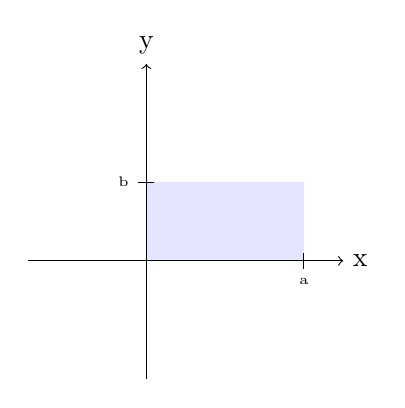
\begin{tikzpicture}
	\coordinate (A0) at (0, 0);
	\coordinate (B0) at (0, 1);
	\coordinate (C0) at (2, 0);
	\coordinate (D0) at (2, 1);
% initial area
\path [fill=blue!10] (A0) -- (B0) -- (D0) -- (C0) -- (A0);
	% les axes
	\draw[->] (-1.5,0) -- (2.5,0) node[anchor=west]{x};
	\draw[->] (0,-1.5) -- (0,2.5) node[anchor=south]{y};
	% tick marks
	\draw[-] (-0.1, 1) node[anchor=east]{\tiny b} -- (0.1, 1);
	\draw[-] (2, -0.1) node[anchor=north]{\tiny a} -- (2, 0.1);
\end{tikzpicture}
\caption{Rectangle d'aire $ab$ engendré par les vecteurs
$\displaystyle \left( a\atop 0\right)$ et
$\displaystyle \left(0 \atop b\right)$.
}
\end{minipage}
\hfill
\begin{minipage}{0.45\textwidth}
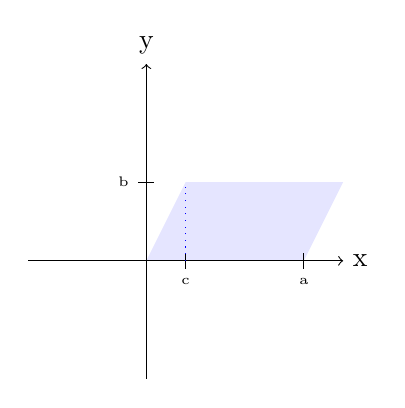
\begin{tikzpicture}
	\coordinate (A0) at (0, 0);
	\coordinate (B0) at (0.5, 1);
	\coordinate (C0) at (2, 0);
	\coordinate (D0) at (2.5, 1);
% initial area
\path [fill=blue!10] (A0) -- (B0) -- (D0) -- (C0) -- (A0);
	% les axes
	\draw[->] (-1.5,0) -- (2.5,0) node[anchor=west]{x};
	\draw[->] (0,-1.5) -- (0,2.5) node[anchor=south]{y};
	% tick marks
	\draw[-] (-0.1, 1) node[anchor=east]{\tiny b} -- (0.1, 1);
	\draw[-] (2, -0.1) node[anchor=north]{\tiny a} -- (2, 0.1);
	\draw[-] (0.5, -0.1) node[anchor=north]{\tiny c} -- (0.5, 0.1);
	\draw[dotted, blue] (0.5, 0) -- (B0);
\end{tikzpicture}
\caption{Parallélogramme d'aire $ab$ engendré par les vecteurs
$\displaystyle \left( a\atop 0\right)$ et
$\displaystyle \left(c \atop b\right)$. À noter que
l'on obtient un tel parallélogramme via une transformation
linéaire de cisaillement (avec un déterminant égal à 1) faite sur
un rectangle d'aire $ab$.
}
\end{minipage}
\end{figure}
Qu'arrive-t-il si l'une des deux colonnes correspond au vecteur nul
ou que l'une des deux colonnes soit un multiple de l'autre?  
Dans ce cas, nous avons effectivement un seul vecteur qui définit
un parallélépipède d'aire nulle.
Finalement, si on interchange deux colonnes, on trouve que le
déterminant change de signe.  Puisqu'une aire est définie
comme étant une valeur positive, lorsqu'on donne une
interprétation géométrique au déterminant, on ignore
simplement le signe.\footnote{En fait, on peut considérer le signe
si on définit des surfaces ou des systèmes d'axes \textit{orientés},
l'orientation changeant de signe lorsqu'on fait une réflexion par
rapport à un axe, par exemple.}

\subsection{Transformations linéaires}
Imaginons que nous avons une surface $S$ correspondant à
un parallélogramme d'aire $A$; nous pouvons
concevoir ce parallélogramme comme étant engendré
par les vecteurs colonnes de la matrice $\matB$ comme on
l'a déjà vu ci-dessus.
Supposons que nous faisions une transformation linéaire $T(S)$,
via la matrice $\matM$,
pour obtenir un nouveau parallélogramme d'aire $A'$. Nous avons
\[
A' = \det(\matM \matB) = (\det\matM)(\det\matB) = (\det\matM) A
\]
Ce résultat se généralise à d'autres formes que les parallélogrammes
si on considère une surface $S$ comme étant une somme (infinie) de
petits rectangles (et que l'on passe à la limite).
\begin{exemple}
Une application intéressante du calcul d'aires est celle
d'une ellipse.  
\[
\frac{x^2}{a^2} + \frac{y^2}{b^2} = 1
\]
Soit un point $\displaystyle \begin{pmatrix}
u\\v
\end{pmatrix}
$
tel que $u^2 + v^2 \leq 1$.  Ce point est
situé à l'intérieur d'un cercle unitaire, d'aire égale
à $\pi$.
Appliquons la transformation linéaire:
\[
\matA = 
\begin{pmatrix}
a & 0 \\
0 & b
\end{pmatrix}
\]
à ce point.
On obtient un point $\displaystyle \begin{pmatrix}
x\\y
\end{pmatrix}
$
situé à l'intérieur de l'ellipse
$\displaystyle
\frac{x^2}{a^2} + \frac{y^2}{b^2} \leq 1
$
Nous avons donc:
$\displaystyle
\mbox{[aire de l'ellipse]} = \begin{vmatrix}
a & 0 \\
0 & b
\end{vmatrix}\mbox{[aire du cercle]} = ab \pi
$
\end{exemple}

\subsection{Dimensions supérieures à deux}
Si au lieu d'un plan, on considère un espace à trois dimensions, 
le déterminant nous donnera le volume du parallélépipède engendré par les
trois vecteurs.  Si le déterminant est nul, cela signifie que
les trois vecteurs (colonnes) sont co-planaires.  
Dans les dimensions plus élevées, on généralise ces notions
et on parle de l'hypervolume engendré par les vecteurs.

Pour les transformations linéaires, si le déterminant est nul, cela veut dire que l'on
a fait une projection sur une, ou plusieurs dimensions.  Par exemple, on a pris des points
dans un espace à trois dimensions et on les a projeté sur un plan.  
En faisant une telle transformation, on perd l'information sur la hauteur relative des points
par rapport au plan sur lequel ils ont été projetés; ceci explique pourquoi une telle transformation
est irréversible.

\begin{TwoCol}
\section{Exercices divers}

\begin{exercice}\label{ex:vandermonde} Calculez
\[
\begin{vmatrix}
1 & 2 & 4 \\
1 & 3 & 9 \\
1 & 5 & 25
\end{vmatrix}
\]
\end{exercice}
\begin{exercice} \label{ex:explicit}
Calculez le déterminant des matrices suivantes.
\partexercice{a}$\displaystyle \begin{pmatrix}
1 & 0 & 0 & 0 & 0 \\
0 & 1 & 0 & 0 & 0 \\
0 & 0 & 1 & 0 & 0 \\
0 & 0 & 0 & 4 & 3 \\
0 & 0 & 0 & 5 & 4
\end{pmatrix}$
\partexercice{b}$\displaystyle \begin{pmatrix}
4 & 4 & 0 & 0 & 0 \\
3 & 5 & 0 & 0 & 0 \\
0 & 0 & 1 & 0 & 0 \\
0 & 0 & 0 & 1 & 0 \\
0 & 0 & 0 & 0 & 1
\end{pmatrix}$
\partexercice{c}$\displaystyle \begin{pmatrix}
1 & 0 & 0 & 77 & -8 \\
0 & 1 & 0 & 9 & 3 \\
0 & 0 & 1 & 24 & 5 \\
0 & 0 & 0 & 4 & 3 \\
0 & 0 & 0 & 5 & 4
\end{pmatrix}$
\end{exercice}
\begin{exercice}
Soit les matrices:
\[
\matA = \begin{pmatrix}
1 & 0 \\ 0 & -1
\end{pmatrix} \qquad
\matB = \matI
\]
\[
\matC = \begin{pmatrix}
0 & 1\\ 1 & 0
\end{pmatrix} \qquad
\matD = \begin{pmatrix}
0 & 1\\ 0 & 0
\end{pmatrix}
\]
\[
\matE = \begin{pmatrix}
\matA & \matB \\ \matC & \matD
\end{pmatrix}
\]
Calculez $\det \matE $ et $\det (\matA\matD - \matC\matB)$.  Est-ce que vous
obtenez le même résultat dans les deux cas?
\end{exercice}
\begin{exercice}
Soit $\matA$ et $\matD$ deux matrices carrées.  En suivant ce que vous avez
fait pour trouver les réponses de l'\refexercice{ex:explicit}, démontrez que
\partexercice{a} $\displaystyle
\det \begin{pmatrix}
\matA & \zero \\
\zero & \matI_n
\end{pmatrix} = \det \matA$
\reponse
Un début de réponse est comme suit:  Comme la matrice $\matA$ est
une matrice une matrice carrée, supposons qu'elle est de taille $m\times m$. 
En faisant l'expansion du déterminant
par la dernière ligne, tous les termes sont zéros sauf un, dont le coefficient
est à la ligne $m+n$ et à la colonne $m+n$ et on trouve
\[
\det \begin{pmatrix}
\matA & \zero \\
\zero & \matI_n
\end{pmatrix} = (-1)^{2m+2n} \det \begin{pmatrix}
\matA & \zero \\
\zero & \matI_{n-1}
\end{pmatrix}
\]
\partexercice{b}  $\displaystyle
\det \begin{pmatrix}
\matI_n & \zero \\
\matC & \matD
\end{pmatrix} = \det \matD$
\partexercice{c} Utilisez les résultats précédents pour démontrer que
\[
\det \begin{pmatrix}
\matA & \zero \\
\matC & \matD
\end{pmatrix} = (\det \matA)(\det\matD)
\]
\partexercice{d}$\displaystyle \det \begin{pmatrix}
\matA & \matB \\
\zero & \matD
\end{pmatrix} = (\det \matA)(\det\matD)$
\end{exercice}
\begin{exercice}
Soit $\matA_{n\times n}$ et $\matD_{m\times m}$ deux matrices carrées. 
Vous pouvez supposer que $\matA^{-1}$ existe.
\partexercice{a} Trouvez les matrices $\matX$ et $\matY$ telles que
\[
\begin{pmatrix}
\matA & \matB \\ \matC & \matD
\end{pmatrix}
= \begin{pmatrix}
\matI & \zero \\ \matX & \matI
\end{pmatrix}
\begin{pmatrix}
\matA & \matB \\ \zero & \matY
\end{pmatrix}
\]
et utilisez ce résultat pour démontrer que
\[
\begin{vmatrix}
\matA & \matB \\ \matC & \matD
\end{vmatrix} = (\det\matA)(\det(\matD-\matC\matA^{-1}\matB))
\]
\partexercice{b} Quelle doit être la valeur de $m$ pour qu'il soit possible d'avoir $\matA\matC = \matC\matA$?
\partexercice{c} Démontrer que, si $\matA\matC = \matC\matA$, alors
\[
\begin{vmatrix}
\matA & \matB \\ \matC & \matD
\end{vmatrix} = \det (\matA\matD - \matC\matB)
\]
\end{exercice}
\begin{exercice}
Soit la matrice $\displaystyle \matA = \begin{pmatrix}
1 & a & a^2 \\
1 & b & b^2 \\
1 & c & c^2
\end{pmatrix}$
qui est un exemple d'une matrice de Vandermonde. En utilisant des opérations sur les lignes,
démontrez que le déterminant de cette matrice peut être écrit sous la forme:
\[
\begin{vmatrix}
1 & a & a^2 \\
1 & b & b^2 \\
1 & c & c^2
\end{vmatrix} = x y \begin{vmatrix}
1 & a & a^2 \\
0 & 1 & a+b\\
0 & 1 & a+c
\end{vmatrix}
\]
Puis, en continuant de faire des opérations sur les lignes, démontrez que
\[
\begin{vmatrix}
1 & a & a^2 \\
1 & b & b^2 \\
1 & c & c^2
\end{vmatrix} = (b-a)(c-a)(c-b)
\]
Vérifiez votre résultat en comparant avec ce que vous aviez obtenu pour l'\refexercice{ex:vandermonde}.
\end{exercice}

% matrice de van der monde

\end{TwoCol}